\documentclass[main.tex]{subfiles}

\begin{document}


\index{IceCube Neutrino Observatory}The IceCube Neutrino Observatory is a gigaton-scale Cherenkov observatory instrumented across a cubic kilometer at the South Pole, two kilometers deep, in the Antarctic glacial ice~\cite{Aartsen_2017}.
As shown in Figure~\ref{fig:icecube_figs} (left) IceCube is composed of 5160 photo-multiplier tubes encased within glass pressure vessels, called ``Digital Optical Modules'' (DOMs)~\cite{ABBASI2009294}, which are used to detect the Cherenkov light emission from the charged daughter-particles resulting from neutrino interactions in and around the detector.
These DOMs are arranged vertically with a seventeen-meter spacing into seventy-nine strings, which themselves are aligned into a hexagonal lattice with a 125-meter spacing. 
A more densely instrumented sub-detector called DeepCore was also installed towards the bottom-center of the main detector~\cite{ABBASI2012615}; the additional strings of this dense in-fill brings the total string count to eighty-six.
Working primarily as a cosmic-ray air shower detector, an array of surface detectors named IceTop is installed on surface of the IceCube glacier.
A schematic illustration of the IceCube string and IceTop tank locations is shown in Figure~\ref{fig:icecube_figs}\footnote{String 37 is off-grid as a result of a sub-surface crate of pork chops obstructing the original drill-site, see Appendix~\ref{app:pork}.}.

\begin{figure}
    \centering
    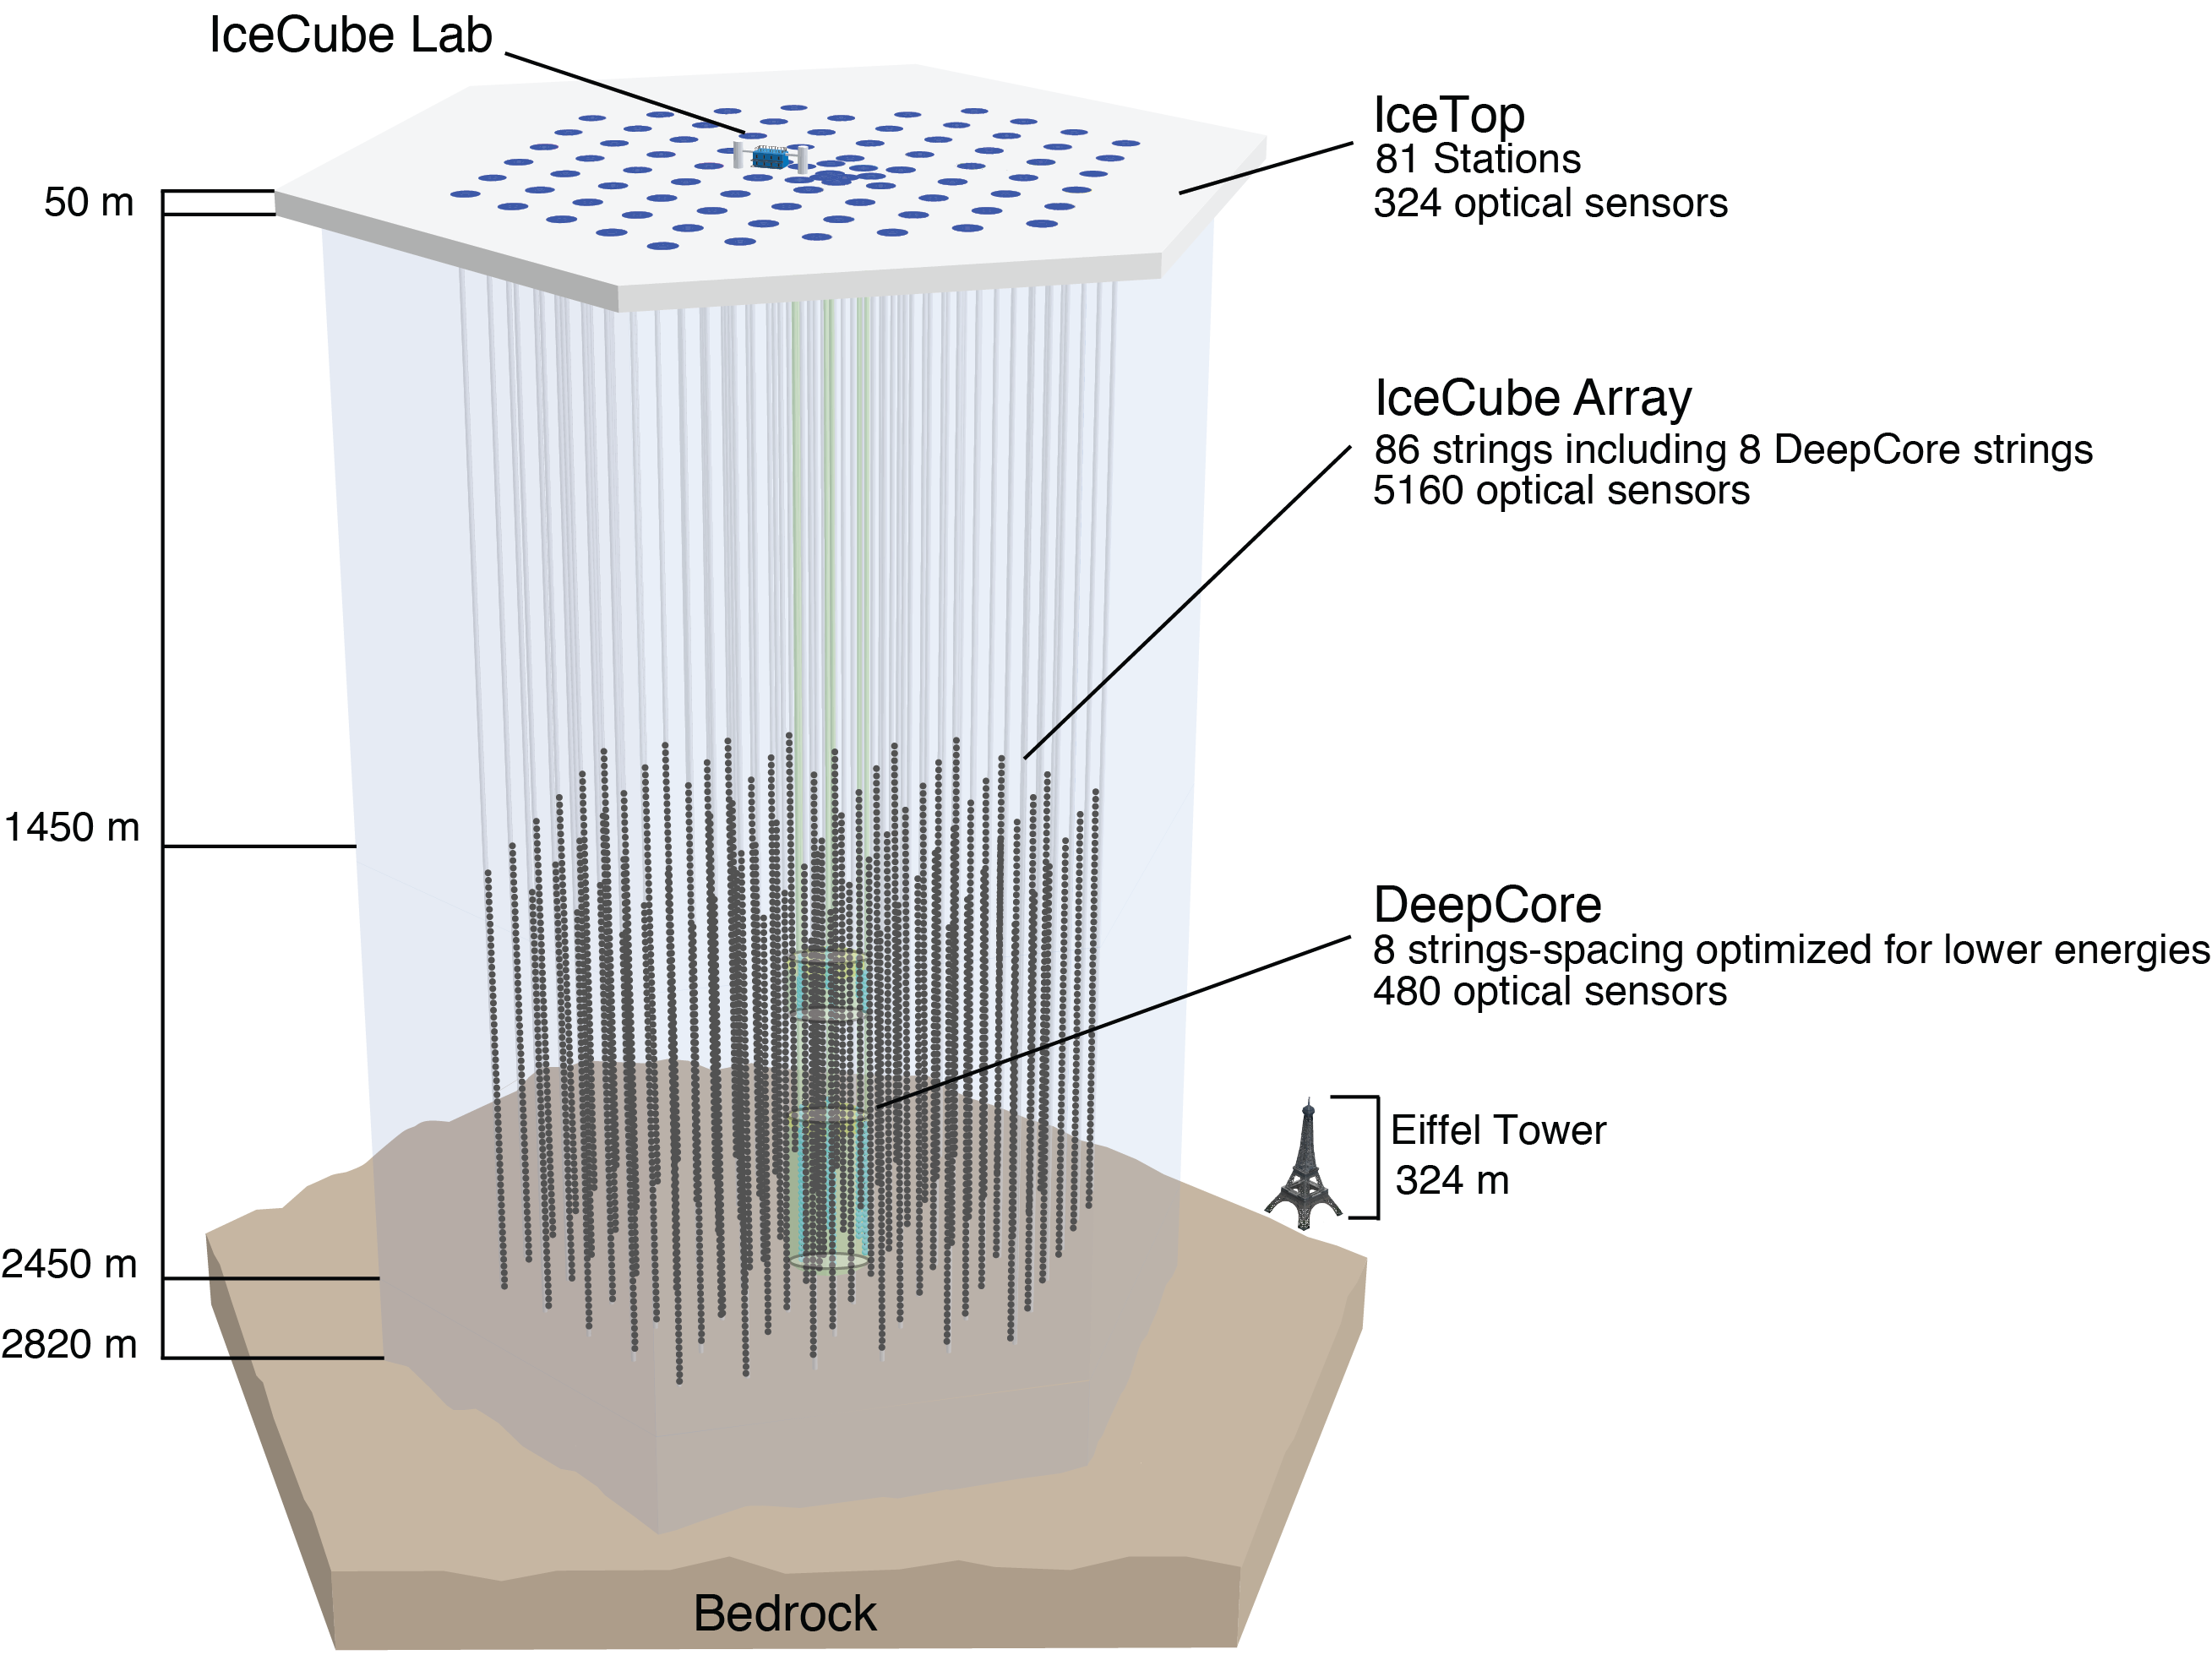
\includegraphics[width=0.5\linewidth]{figures/IceCubeArray.png}
    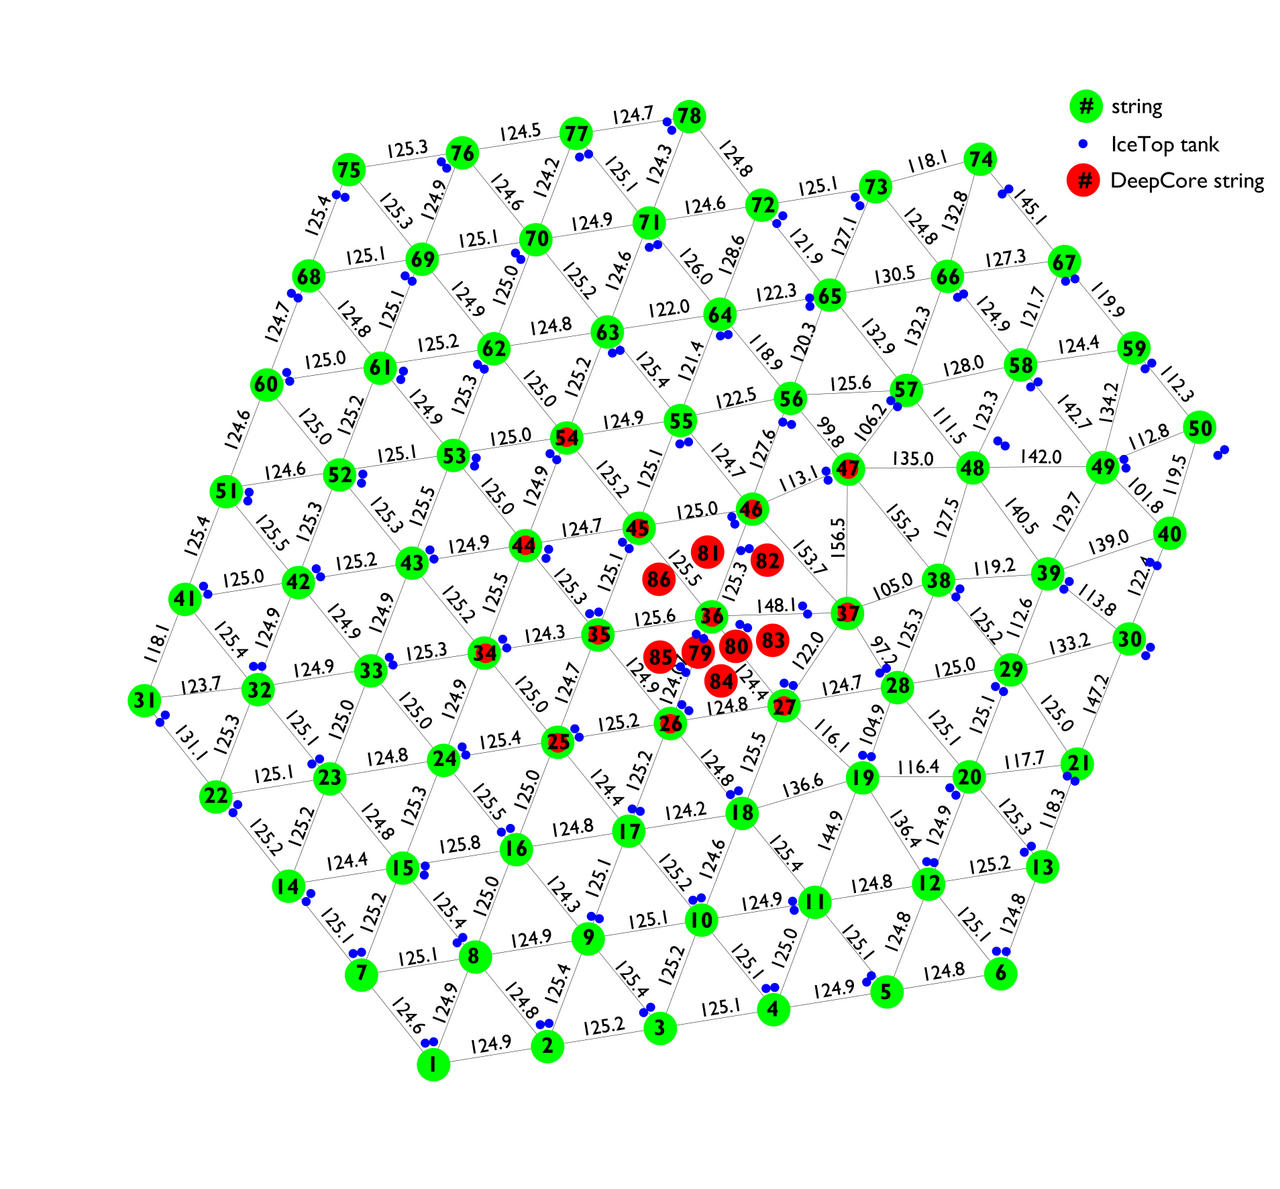
\includegraphics[width=0.4\linewidth]{figures/VetoView2_distance_123012.jpg}
    \caption{Left: a side-view of the IceCube Neutrino Observatory detector array, showing the span of the instrumented volume and DeepCore, plus the IceCube Lab and IceTop on the surface. The IceCube Lab is not to scale. Right: a top-down schematic showing the distribution of IceCube and DeepCore strings and the distances between them.}\label{fig:icecube_figs}
\end{figure}

\section{Event topologies}\label{sec:event_morphology}

Large-volume neutrino telescopes, like IceCube, typically are sensitive in the TeV to PeV energies; here, Deep-Inelastic Scattering (DIS)~\cite{gandhineutrinos} interactions dominate, and Glashow Resonance~\cite{PhysRev.118.316} interactions have only just been observed~\cite{IceCube:2021rpz}.
The detected neutrino interaction events fall into two morphological categories: tracks and cascades.

Charged-current (CC) $\nu_{\mu}$ DIS events result in muons at energies where radiative processes dominate energy loss rates.
As a result, energy losses are stochastically driven and the produced muons travel for kilometers. 
The consequences are threefold: muons are difficult to fully contain in neutrino telescopes, muon energies are poorly correlated with progenitor muon-neutrino energies, and muons' long travel-distance can allow for reconstructing their direction to within 1$^{\circ}$~\cite{trackaccuracy2017}. These events are called \textit{tracks}~\cite{icecube_energy_reco}.

All neutral-current (NC) DIS events result in a hadronic shower spreading around the interaction point and a secondary neutrino invisibly carrying away a proportion of the parent neutrino's energy. 
These events are often contained with a roughly spherical topology. 
$\nu_{e}$-CC interactions develop similarly to neutral-current interactions, but repeated inverse Compton scattering of the produced electron initiates an electromagnetic shower superimposed over the hadronic shower. 
Thus, nearly all of the interacting neutrino's energy is observable as detectable light. 
These events are called \textit{cascades.} Such events tend to be well-contained permitting an efficient energy reconstruction, although they suffer from poor angular reconstruction~\cite{icecube_energy_reco}. 

The evolution of a $\nu_{\tau}$-CC interaction is highly dependent on the energies involved. A tau is produced simultaneously as a hadronic cascade propagates around the interaction point, and then the tau decays. 
Due to their large mass, taus have a short lifetime and a decay length of $\sim 50$ m per PeV of tau energy~\cite{abbasi2020measurement}. 
From the tau branching ratios~\cite{PhysRevD.98.030001}, 17.37\% of the charged tau decays evolve as muon tracks, while the remainder of the decays evolve as electromagnetic or hadronic cascades. Only at neutrino energies above 60 TeV do $\nu_{\tau}$-CC interactions yield events with potentially distinguishable primary and secondary cascades~\cite{abbasi2020measurement}; at lower energies the secondary cascade is indistinguishable from the hadronic one. Tau events which decay into muons will appear as starting track events while the remainder appear as cascades. 

\iffalse
Several distinct event samples have been developed to study these different types of events in IceCube. The High-Energy Starting Events sample~\cite{2021hese}, for example, was developed to study both taus and high-energy neutrinos likely astrophysical in origin. There exist other events samples optimized for higher event rates at lower energies, such as the Medium-Energy Starting Events~\cite{PhysRevDoverone}, and the five-year inelasticity sample~\cite{inelasticity2019}. There are also samples optimized for muon purity, such as the eight-year atmospheric muon sample~\cite{Aartsen_2020_prd} and others optimized for accurate energy resolution such as the six-years cascade sample~\cite{sixyrscascade}. This work will consider the cascade event selection described in~\cite{2018PhDT17N} and the track event selection previously used in IceCube sterile neutrino searches~\cite{Aartsen_2020, Aartsen_2020_prd}.
\fi

\section{The Ice}\label{sec:the_ice_stuff}
As discussed in Ref~\cite{journal_glaciology_2013}, the Antarctic ice containing IceCube is a rapidly-moving\footnote{several meters per year} glacier formed over hundreds of thousands of years of compacted snowfall. 
The first few hundred meters, known as the \textit{firn} layer, is an opaque layer of geologically new snow. 
At greater depths the integrated weight of the snow overburden compresses the firn layer snow into an ice characterized by short scattering lengths ($\mathcal{O}$(meters)) dominated by trapped bubbles of air.
At even greater depths, the pressures reach an extreme enough level such that the ice enters a new crystalline phase along with the air molecules. 
The resulting, \textit{clathrate} ice boasts good optical properties, where the optical defects are characterized instead by microscopic grains of dust and pollutants.
Scattering lengths at these depths are on the order of 10s of meters while the absorption lengths rise to 100s of meters. \index{ice!bulk}
Layers formed at the same point in time, or isochrons, tend to have similar ice optical properties as a result. 

\begin{figure}
    \centering
    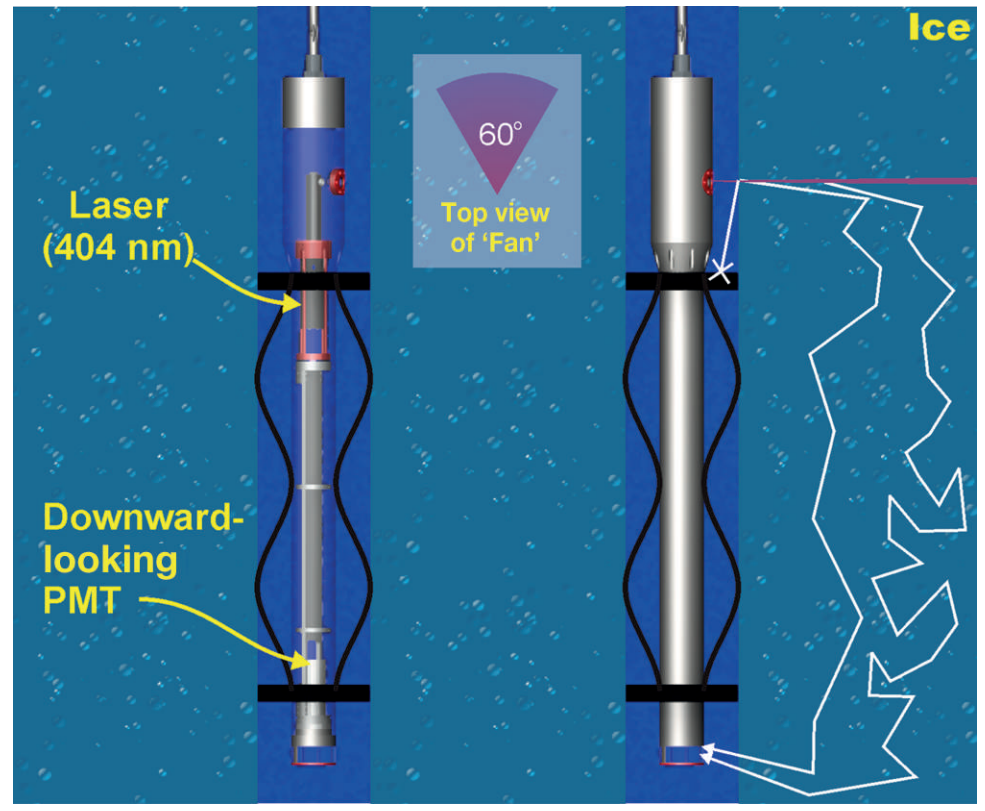
\includegraphics[width=0.6\linewidth]{figures/dustlog.png}
    \caption{A diagram of the IceCube dust logger.}\label{fig:dustlog}
\end{figure}

The properties were studied during the deployment of IceCube using a \textit{dust logger}, a long, ruggedized, device with a fan-shaped 404 nanometer diode laser that could probe a 60 degree wide field of view. 
It used a downward-looking PMT at the bottom of the device to measure the intensity of back-scattered light.
This device was lowered down six of the eighty-six boreholes dug during the IceCube deployment, which are shown on the right of Figure~\ref{fig:icetilt}.
A diagram of the dust logger is shown in Figure~\ref{fig:dustlog}.

\begin{figure}  
    \centering
    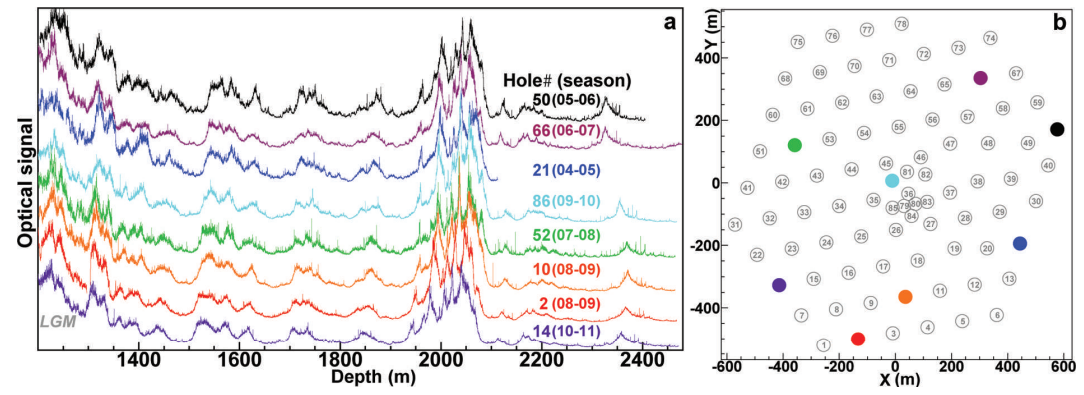
\includegraphics[width=0.8\linewidth]{figures/tilt.png}
    \caption{On the right we show which of the eighty-six boreholes dust-logger data was taken, and on the left we show the intensity of the back-scattered light as measured at each of the sampled holes as a function of depth.}\label{fig:icetilt}
\end{figure}

Data from the dust logger, shown in Figure~\ref{fig:icetilt}, demonstrate that the absorption length and scattering length vary greatly as a function of depth. 
The depth-profiles also varied slightly from hole-to-hole: suggesting ice at similar depths, but separated laterally, did not have the same optical properties.

As the glacier around the present day location of IceCube moved and formed over hundreds of thousands of years, the pressures of the ice over the hard bedrock beneath it warped and bent the glacier. 
The result of this is that the layers of ice with similar optical properties are not flat layers, but tilted and warped. \index{ice!tilt}
Uncertainty in the bulk ice properties and their impacts on analysis-level quantities are discussed in Section~\ref{sec:bulk}.

\begin{figure}  
    \centering
    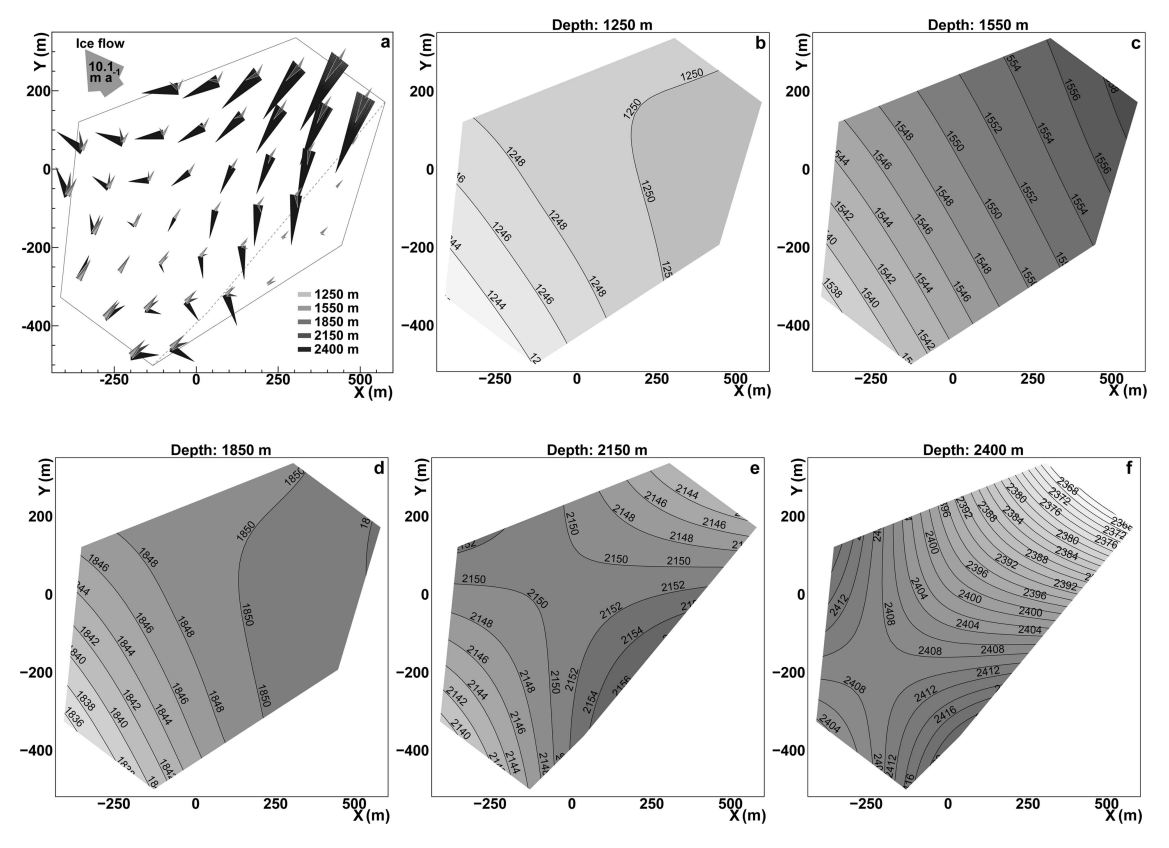
\includegraphics[width=0.8\linewidth]{figures/icecube_isochron.png}
    \caption{(a) shows the flow direction of the South Pole glacier (b-f) Cross-sections of the ice at various depths showing contours for different isochrons: demonstrating the tilt of the ice.}\label{fig:isochron}
\end{figure}

As the borehole water refroze around the IceCube strings, it froze inwards from the glacial wall. 
This drew in trapped air from the clathrate air, resulting in a column of bubbles which formed in the central 5-10 cm of each borehole.
This bubbly ``hole ice'' results in a much shorter scattering length when compared to the bulk ice in the region around the DOMs. 
The models which describe it, and its impact on analysis quantities, are described in Section~\ref{sec:hole_ice}. 

During one of the dust-logger ascents, it was observed to smoothly rotate at a rate of one revolution per 25 meters depth. 
Below 1100 meters, a consistent intensity in the back-scattered light was observed when the fan-laser was aligned with the direction of the glacial flow. 
Later in-ice studies attributed the optical anisotropy to a process where the flow of the glacial ice induced a shear between ice crystal grains and reorienting them to be orthogonal to the flow axis. 
The ice crystals became birefringent, such that light diffusion is greatest along the flow axis, and light would deflect towards the flow axis~\cite{ice_anisotropy, ice_birefringence}.
Only some newer, internal, IceCube ice models account for the birefringence. 
Legacy models, like \textbf{S}outh \textbf{P}ole \textbf{ICE} 3.2.1 (Spice 3.2.1), are still widely used for analyses.
Newer models, like \textbf{B}ire\textbf{FR}ingence v2 (BFR v2), are slowly being adopted by other analyses where it is shown that birefringence is found to be a relevant effect. 
This adoption is slowed, however, by the expensive cost of re-generating Monte Carlo samples with the updated ice models and by the need to then validate changes to the simulation. 

\section{\v{C}erenkov Radiation}

As charged particles move through ice (or any transparent media), due to dielectric effects the particles themselves can move faster than the phase velocity of the light within it. 
The particle will collectively polarize molecules in the surrounding bulk as it passes, and as these molecules relax to their original orientations. 
This manifests as the emission of light in the shape of a cone opening outwards into the direction of the particle's propagation: \v{C}erenkov Radiation. 

The threshold above which this happens can be found from energy-momentum relationships with a velocity substitution of the 3-momentum, or 
\begin{equation}
    E^{2} = m^{2} + \dfrac{m^{2}v^{2}}{1-v^{2}}.
\end{equation}
We then consider a transparent material with an index of refraction $n = 1./v_{critical}$, where $v$ is the phase velocity light in the medium. 
Particles travelling at a velocity at or above this threshold will emit \v{C}erenkov radiation. 
The associated energy $E_{critical}$ can be solved for algebraically,
\begin{align}
        E^{2}_{critical} &= m^{2} + \dfrac{m^{2}v_{critical}^{2}}{1-v_{critical}^{2}} \\
        E^{2}_{critical}  - m^{2} - E^{2}_{critical}v_{critical}^{2}  + m^{2}v_{critical}^{2} &= m^{2}v_{critical}^{2} \\
        E^{2}_{critical}\left(1  -v_{critical}^{2}\right) &=  m^{2} \\
        \sqrt{\dfrac{m^{2}}{\left(1  -n^{-2}\right)}} &= E_{critical} 
\end{align}

Like a sonic boom of light, the light is emitted in a cone which opens at an angle $\theta_{c}$ relative to the direction at which the particle travels. 
This angle is given by
\begin{equation}
\tan\theta_{c} = \sqrt{v^{2}n^{2} - 1} .
\end{equation}
Although the light is emitted in the forward direction, the \v{C}erenkov light wave-front counter-intuitively trails in a cone opening behind the radiating particle. 

For highly relativistic particles travelling through ice, this angle is $41^{\circ}$, and the emitted light ranges from 300 to 600 nm. 


\section{The Digital Optical Modules}

IceCube's Digital Optical Modules, or DOMs, are composed of a 0.5'' thick borosilicate glass pressure vessel with a downwards-facing 10'' Hamamatsu R7081-02 PMT and an onboard computer mounted internally on the DOM mainboard.
The PMT has single-photon sensitivity in the 300-650 nm range with a 25\% peak quantum efficiency at 390 nm~\cite{ABBASI2010139}.
The PMT is optically connected with the glass pressure vessel using gel to maximize transmittance of light through the vessel and into the PMT; it is protected from the Earth's magnetic field via a mu-metal wire mesh. 
The DOM's onboard computer houses the electronics and software necessary to trigger the DOM on any signal incident upon the PMT. 
A schematic design of a DOM is shown in Figure~\ref{fig:dom_design}. 


\begin{figure}
    \centering
    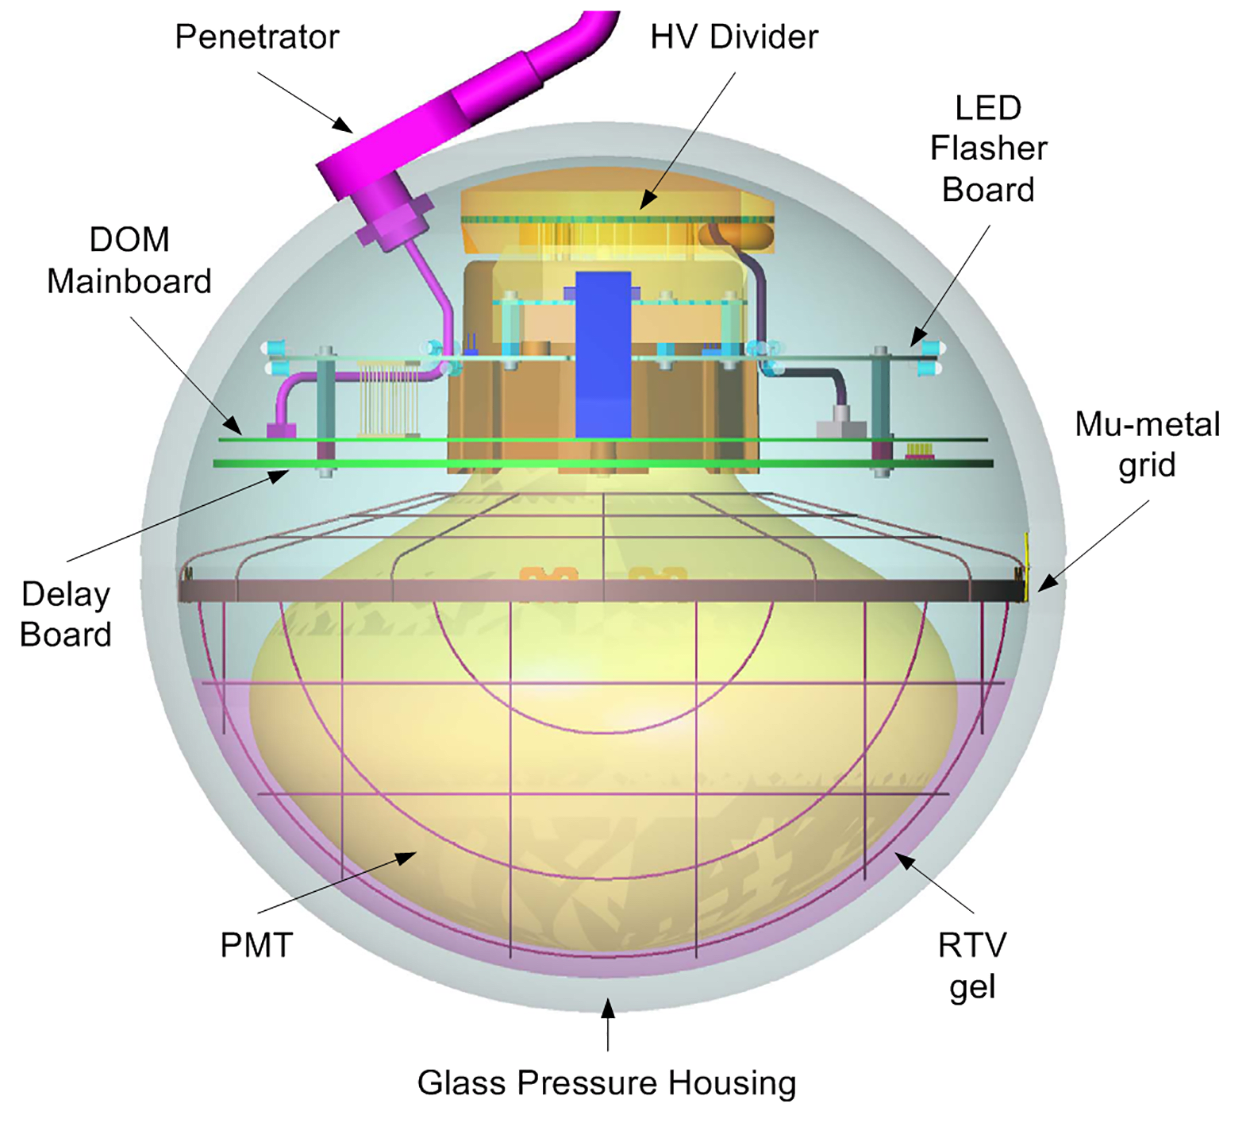
\includegraphics[width=0.8\linewidth]{./figures/icecube_dom.png}
    \caption{A schematic of a Digital Optical Module (DOM).}\label{fig:dom_design}
\end{figure}

\section{Data Acquisition}

When a DOM's PMT reads sufficient charge to cross the single-photon threshold, the DOM is triggered and signal collection starts. 

To minimize spurious detector triggers a coincidence threshold trigger is used. 
Upon DOM triggering, DOMs communicate directly with their neighbors, and if any neighboring DOMs are triggered within a 1$\mu$s window, a ``hard local coincidence'' (HLC) occurs.
After an HLC, the surface-based IceCube Lab (ICL) registers a `hit' and the DOMs transmit their trigger timing information and full PMT waveforms.
At the ICL a Simple Multiplicity Trigger (SMT) is applied: if eight\footnote{Starting in 2024 runs, this threshold is changing to twelve} HLC hits or more are detected in a 5$\mu$s window, a global detector trigger occurs and the trigger window is extended until another 5$\mu$s window passes with no further HLC hits neighboring the DOM hits. 
At this point, the global detector trigger rate is approximately 2kHz and the raw data output is around 1 TB/day. 
This data rate is too large, and so, all hits within the time window are collected into an Event and passed to the ICL ``Processing aNd Filtering'' (PnF) system in order to reduce the data volume below the amount allocated for IceCube's satellite collection (100 GB/day). 
A rudimentary reconstruction is run to calculate an approximate event interaction vertex, direction, and energy. 
About 25 separate filters are then applied on these reconstructed event values to select only those Events of interest for ongoing IceCube analyses: if any trigger passes then the event is kept, processed further, and transmitted to the North\footnote{Anywhere that isn't Antarctica: the \textit{North} usually refers to Madison, Wisconsin, however.}. 
Each filter is carefully studied before implementation, analyzers must provide predictions for the expected data bandwidth, CPU core-hours of processing required, data storage requirements, and extensive testing of the software responsible for running the trigger. 
Approximately 15\% of all events are selected by one or more filter~\cite{Aartsen_2017}. 

\end{document}